\section{Static equilibrium}
In this section we explain the mathematical fundamentals as well as the model used to capture differential thrust. The equation of flights in aerodynamic frame are first re-called, then modeling of propulsion is shown and finally the trimming algorithm is explained.

\subsection{Equation of flight}
The equations of flight in the aerodynamic frame, assuming uniform wind velocity are used. This form is the most commonly used when studying the lateral flight dynamics. Equations are taken from Boiffier \cite{Boiffier} and are equivalent to those presented by Goman in\cite{GomanAttainableEqui}:
\begin{align}
	\begin{pmatrix}
	m \dot{V} \\
	m\left[ \dot{\beta}V -V(p\sin\alpha - r\cos\alpha) \right]\\
	m\left[ \dot{\alpha} V \cos\beta + V\left(\sin\beta (p\cos\alpha + r\sin\alpha) - q\cos\beta\right)\right]
	\end{pmatrix}
	= & mg
	\begin{pmatrix}
	-\sin\gamma\\
	\cos\gamma \sin\mu\\
	\cos\gamma \cos\mu	
	\end{pmatrix}
	+ \frac{1}{2} \rho S V^2
	\begin{pmatrix}
	-C_D\\
	C_Y\\
	-C_L
	\end{pmatrix}
	+ \mathbf{H_{ab}} 
	\begin{pmatrix}
	F_{x_b}\\
	F_{y_b}\\
	F_{z_b}
	\end{pmatrix} \label{E:Sdtdebut}\\
	\textbf{I}
	\begin{pmatrix}
	\dot{p}\\
	\dot{q}\\
	\dot{r}
	\end{pmatrix}
	 + \begin{pmatrix}
	 p\\
	 q\\
	 r
	 \end{pmatrix} \times \textbf{I}
	 \begin{pmatrix}
	 p\\
	 q\\
	 r
	 \end{pmatrix}
 	 =& \frac{1}{2} \rho S V^2 l
	\begin{pmatrix}
	C_l\\
	C_m\\
	C_n
	\end{pmatrix}
	+
	\begin{pmatrix}
	M_{x_b}\\
	M_{y_b}\\
	M_{z_b}
	\end{pmatrix} \label{E:sdtMoments}
\end{align}

Where \textbf{I} is the inertia matrix, $\mathbf{H_{ab}}$ is the rotation matrix from body to aerodynamic frame projecting forces ($F_{x_b}$,$F_{y_b}$,$F_{z_b}$) due to propulsion:

\begin{align}
H_{ab} =& 
\begin{pmatrix}
\cos\alpha \cos\beta & sin\beta & \sin\alpha \cos\beta\\
-\cos\alpha \sin\beta & \cos\beta & \-sin\alpha \sin\beta\\
-\sin\alpha & 0 & \cos\alpha 
\end{pmatrix}
\end{align}

The weight is projected onto the aerodynamic airframe through the climb angle $\gamma$ and the aerodynamic bank angle $\mu$. These terms can be expressed as \cite{Boiffier}:
\begin{align}
\cos\gamma \sin\mu =& \sin\theta \cos\alpha \sin\beta + \cos\beta\cos\theta\sin\phi - \sin\alpha\sin\beta\cos\theta\cos\phi\\
\cos\gamma \cos\mu =& \sin\theta\sin\alpha + \cos\beta\cos\theta\cos\phi
\end{align}

The complementary kinematic equations are :

\begin{align}
\begin{pmatrix}
\dot{\phi}\\
\dot{\theta}\\
\dot{\psi}
\end{pmatrix}
= \begin{pmatrix}
1 & \sin\phi \tan\theta & \cos\phi \tan\theta\\
0 & \cos\phi & -\sin \phi\\
0 &\frac{\sin\phi}{\cos\theta} & \frac{\cos \phi}{\cos \theta}
\end{pmatrix}
\begin{pmatrix}
p\\
q\\
r
\end{pmatrix} \label{E:kinematics}
\end{align}

Additional parameters, namely the climb angle $\gamma$ and the turn rate $\Omega$ are definied as :
\begin{align}
\sin \gamma &= \cos\alpha\cos\beta\sin\theta - \sin\beta\sin\phi\cos\theta - \sin\alpha\cos\beta\cos\phi\cos\theta \label{E:gammaDef}\\
\Omega &= -\dot{\phi}\sin\theta + \dot{\psi} \label{E:OmegaDef}
\end{align}

The heading variable $\psi$ is of no interest for our study, in order to remove its contribution, we can replace the expression of $\dot{\phi}$ and $\dot{\psi}$ in equation (\ref{E:OmegaDef}) and obtain:
\begin{equation}
\Omega = \left( q \sin \phi + r \cos \phi \right) \sec \theta \label{E:OmegaUse}
\end{equation}

Leaving the heading angle aside, equations (\ref{E:Sdtdebut}), (\ref{E:sdtMoments}), (\ref{E:kinematics}), (\ref{E:gammaDef}) and (\ref{E:OmegaUse}) represent a set of $N_e=10$ equations to satisfy. The state vector is $\textbf{x}=[V,\alpha,\beta,p,q,r,\phi,\theta]$ and counts $n_x=8$ variables. The input vector corresponding to control surfaces, respectively ailerons, elevator and rudder is $\textbf{u}=[\delta_a, \delta_e, \delta_R]$ with $n_u=3$ variables. Finally we count $n_p=2$ additional parameters $\gamma$ and $\Omega$. The model is now ready to be complemented with a model of distributed propulsion.

\subsection{Propulsion modeling}

Propulsion and differential thrust are modeled together and are assumed to only contribute to generating forces and moments. Meaning that the rotor terms or gyroscopique effects are let aside such that equations of flight aren't further modified.
By summing the thrust forces and moments based on the geometrical arrangement shown in Fig~\ref{fig:AmpereTop} :
\begin{align}
\begin{pmatrix}
Fx_b\\
Fy_b\\
Fz_b
\end{pmatrix}
=
\begin{pmatrix}
\sum_{i=1}^{N} T_{x,i}\\
0\\
0
\end{pmatrix}
\text{ and }
\qquad
\begin{pmatrix}
Mx_b\\
My_b\\
Mz_b
\end{pmatrix}
=\begin{pmatrix}
0\\
0\\
\sum_{i=1}^{N} -T_{x,i} y_i
\end{pmatrix}
\end{align}

\begin{figure}[hbt!]
	\centering
	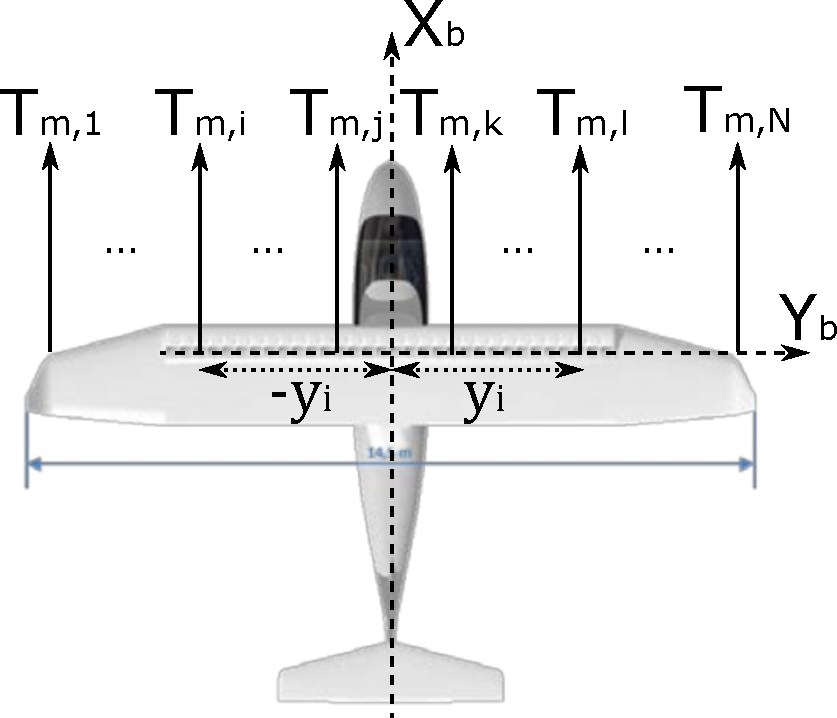
\includegraphics[width=.6\textwidth]{AmpereTop}
	\caption{Illustration of thrust distribution.} Point forces are considered symmetrically placed along the wing. Unlike the configuration of Ampere \cite{Ampere_concept}, equal repartition of engine from root to wing-tip is assumed. \label{fig:AmpereTop}
\end{figure}

Where $T_{x,i}$ and $y_i$ are respectively the thrust force and distance between the body X axis and the i$^{\text{th}}$ motor. 
Our study has previously been limited to propulsive system based on electric engine running propellers. For aircraft equipped with a propeller or a fan, a common thrust model can be \cite{SachsElectricPerf}:
\begin{equation}
	T=PV^{-1} \eta_p \frac{\rho}{\rho_0} \delta x \label{Eq:oldThrustModel}
\end{equation}
Where P is the engine power at sea level, V is the flight velocity, $\eta_p$ is the propeller or fan efficiency, $\rho$ the air density and $\delta_x$ the throttle command. Equation (\ref{Eq:oldThrustModel}) models the loss of power of air breathing engines with variation of air density. Electric motors on the contrary, do not suffer from rarefaction of air as turbomachines, such that we may concider the following thrust model for computing $T_{x,i}$ \cite{SachsElectricPerf}:
\begin{equation}
	T_{x,i}=\frac{P_E}{N}V^{-1}\eta_m\eta_p \delta_{x,i}
\end{equation}
With $P_E$ being the total electrical power available from the line, $N$ being the total number of engine, $\eta_m$ and $\eta_p$ respectively the engine and propeller efficiency (both concidered constant). Hence, we concider that the power is equally divided between each engine. Finally, $\delta_{x,i}$ is the throttle command of each engine and is added to the control input vector : $\textbf{u}=[\delta_a , \delta_e , \delta_R , \delta_{x,1} , \dots , \delta_{x,N}]$. The number of input becomes : $n_u=N_m+3$.

One may argue that electric propulsion will be impacted by altitude anyway. It is true in many aspects, for example:
\begin{itemize}
	\item With increasing altitude cooling of electric engine and power electronics can become more difficult
	\item Maximum rated voltage of conductors decreases with altitude due to Corona effect \cite{WiringSpace}
	\item Finally, in the case of series hybrid or turbo-electric propulsion, the turbo-machine producing the electric power remains sensible to air rarefaction.
\end{itemize}

These limitations are either due to technological locks that can be overcome with increasing interest in electric propulsion or associated with a level of details outside the scope of our study. For these reasons, we will keep the assumption that engine power is constant with altitude.

\subsection{Finding the trim position by optimization}

Similarly to what is done in \cite{GomanAttainableEqui}, a set of additional constraints $N_c$ can now be defined to condition the problem such that only one possible solution exists. The number of variables to determine ($n_x+n_u+n_p$) must equal the number of equations and constraints $N_e+N_c$.
In this case, considering that the number of engine varies, the number of additional constraints to define is given by:
\begin{align}
N_c=&n_x+n_u+n_p-N_e\\
N_c=&N_m+3
\end{align}

In the case where differential thrust is not used, the additional input is $N_m=1$, representing forward thrust or throttle level, and one must fix $N_c=4$ additional constraints, similarly as in \cite{GomanAttainableEqui}. These additional constraints are added to determine the flight condition, typically fixing the following variables: $[V,\beta,\gamma,\Omega]$. With differential propulsion, the minimum number of additional input is $N_m=2$ with two engines. Consequently, the problem becomes quickly overdetermined. An infinite number of equilibrium points can exist. This can be pictured by the different possible combination of throttle level and rudder action to satisfy a certain thrust and yaw moment.

For overdetermined problems, it is common to use optimization methods to find a satisfying solution \cite{OppeinheimerControlAllocation}. Two options are possible: one may define the input vector as $\mathbf{u}=[\delta_a,\delta_e,\delta_n, \delta_x]$ with $\delta_n$ being the total yaw moment input and $\delta_x$ the total thrust force such that the equilibrium problem is well conditioned and then use an optimization method to find the $\delta_R$ and $\delta_{x,i}$. Or one could run the optimization on the complete set of variables. We selected the second option for this study. This is motivated by the will of maintaining a tight coupling between flight dynamics and differential thrust.

It should be stressed that the first option leaves room for development of 
\begin{itemize}
	\item Generic control and allocation laws
	\item Optimal control
	\item Optimisation of design
\end{itemize}

These aspects will be the object of future studies.

Without loss of generality, additional higher and lower bounds are added on control inputs, angle of attack and bank angle depending on the flight phase. For example, the bank angle is limited to $\pm5\degree$ when studying engine failure at take off as stated by flight regulation \cite{CS25}. These bounds are resumed in table \ref{tab:Bonds} and are in part, dependent on the aircraft selected for the study.

The following variables are chosen to imposed the flight conditions $[V,\beta,\gamma,\Omega]$. The objective function to minimize is defined as the power required to maintain equilibrium. Such an objective function makes sense in the point of view of the designer who will look for minimizing the power to install on the aircraft. Finally, to simulate engine failure we simple add a constraint on the throttle level of the corresponding engines.

The problem hence writes:
\begin{align}
\underset{\tilde{x}}{min} & \: \:\sum_{i=1}^{N} T_{x,i} V\\
\text{With:}\qquad \tilde{x}&=[\alpha, p, q, r, \phi, \theta, \delta_a, \delta_e, \delta_R, \delta_{x,1}, \dots, \delta_{x,N}]\\
\text{Subjected to: }&\notag \\
\begin{pmatrix}
0 \\
-mV(p\sin\alpha - r\cos\alpha)\\
mV\left[\sin\beta (p\cos\alpha + r\sin\alpha) - q\cos\beta\right]
\end{pmatrix}
= & mg
\begin{pmatrix}
-\sin\gamma\\
\cos\gamma \sin\mu\\
\cos\gamma \cos\mu	
\end{pmatrix}
+ \frac{1}{2} \rho S V^2
\begin{pmatrix}
-C_d\\
C_Y\\
-C_L
\end{pmatrix}
+ \mathbf{H_{ab}} 
\begin{pmatrix}
\sum_{i=1}^{N} T_{x,i}\\
0\\
0
\end{pmatrix} \\
0 =& \frac{1}{2} \rho S V^2 l
\begin{pmatrix}
C_l\\
C_m\\
C_n
\end{pmatrix}
+
\begin{pmatrix}
0\\
0\\
\sum_{i=1}^{N} T_{x,i} y_i
\end{pmatrix} -
\begin{pmatrix}
p\\
q\\
r
\end{pmatrix}
\times \textbf{I}
\begin{pmatrix}
p\\
q\\
r
\end{pmatrix}\\
0= & p + q\sin\phi \tan\theta + r \cos\phi \tan\theta\\
0= & q\cos\phi -r\sin \phi\\
\Omega = & \left( q \sin \phi + r \cos \phi \right) \sec \theta \\
\sin \gamma = & \cos\alpha\cos\beta\sin\theta - \sin\beta\sin\phi\cos\theta - \sin\alpha\cos\beta\cos\phi\cos\theta\\
0 = & \delta_{x,1}\\
\vdots\notag\\
0 = & \delta_{x,j}
\end{align}

The problem being now defined, the next section will detail the construction of the aerodynamic database as a function of VT area and flight phase.

\begin{table}[hbt!]
	\caption{\label{tab:Bonds} Additional bounds depending on flight phase}
	\centering
	\begin{tabular}{l|c|c|c}
		Flight phase & $V<71 m.s^{-1}$& $V>71 m.s^{-1}$ & Engine failure\\
		\hline
		$\alpha (\degree)$ & $-2\leq\alpha\leq 10$ & $-2\leq\alpha\leq 15$ & (-) \\
		$\phi (\degree)$ & $\pm 30$ & $\pm 30$ & $\pm 5$\\ 
		$\theta (\degree)$ & $\pm 30$ & $\pm 30$& $\pm 30$\\
		$\delta_a(\degree)$ & $\pm 20$& $\pm 20$& $\pm 20$\\
		$\delta_e(\degree)$ & $\pm 20$ & $\pm 20$ & $\pm 20$\\
		$\delta_R(\degree)$ & $\pm 25$ & $\pm 25$ & $\pm 25$\\
		$\delta_{x,i}$ & $0< \delta_{x,i} \leq 1$ & $0< \delta_{x,i} \leq 1$ & $0< \delta_{x,i} \leq 1$ \\
	\end{tabular}
\end{table}

